% !TeX root = ../tesis.tex


\chapter{Eritrocito sano}

\label{section:apendix3}

En la Sección \ref{section:Res_Eritrocito_Sano} se discutieron los resultados obtenidos de $Q_{\text{ext}}$ y del patrón de esparcimiento para $\lambda=431$ nm, asociada al mínimo de la banda de Soret. En esta sección se presentan los resultados para las longitudes de onda representativas de las bandas $\beta$ y $\alpha$. En la Fig.~\ref{subfig:FF_541_health} se muestra la sección transversal diferencial de esparcimiento $\dd{C_{\text{sca}}}/\dd{\Omega}$, así como su representación polar [Fig. \ref{subfig:FF_polar_541_health}] para los cortes $\varphi=0^{\circ}$ y $\varphi=90^{\circ}$ para $\lambda=541$ nm. En la Fig. \ref{fig:FF_cartesian_541_health} se muestra la representación cartesiana de $\dd{C_{\text{sca}}}/\dd{\Omega}$ para los cortes $\varphi=0^{\circ}$ y $\varphi=90^{\circ}$ para $\lambda=541$ nm. Al igual que para $\lambda=431$ nm, el esparcimiento se concentra predominantemente en la región frontal, con un factor de anisotropía de $g=0.98$. Por otra parte, la diferencia entre los cortes $\varphi=0^{\circ}$ y $\varphi=90^{\circ}$ continúa localizándose principalmente en la región lateral, donde la correlación disminuye a $r=0.49$. 
	%
\begin{figure}[h!]
	\centering
	\sidesubfloat[First image]{\hspace{-0.5cm}{	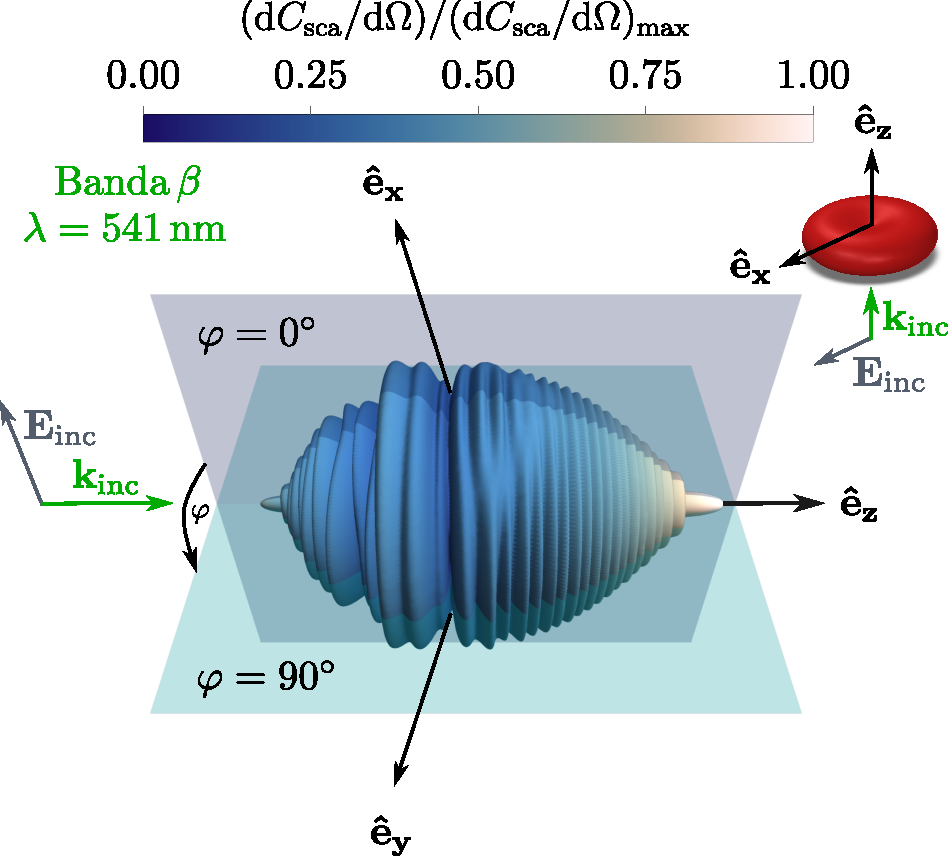
\includegraphics[width=7.3cm]{../../Figuras/4-Resultados/FFdistribution541_EriSano.pdf}\label{subfig:FF_541_health}}}\hspace{0.1cm}
	\sidesubfloat[Second image]{\hspace{-0.5cm}{
			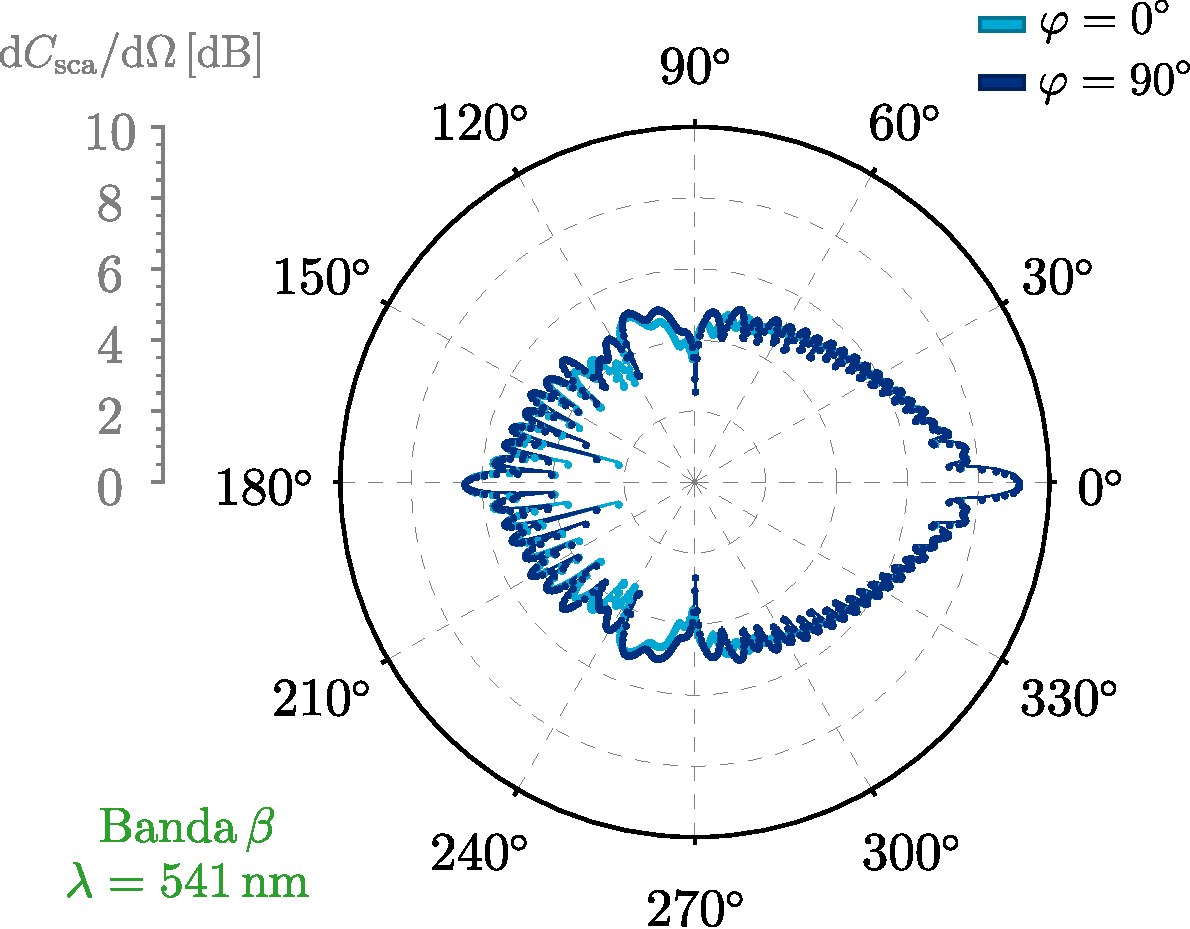
\includegraphics[width=8cm]{../../Figuras/4-Resultados/polarplot541FF_EriSano.pdf}\label{subfig:FF_polar_541_health}}}\vspace{-0.1cm}
	\caption{\textbf{a)} Sección transversal diferencial de esparcimiento $\dd{C_{\text{sca}}}/\dd{\Omega}$ normalizada respecto a su valor máximo para una longitud de onda $\lambda=541$ nm en función del ángulo de esparcimiento $\theta$ y del ángulo $\varphi$ para un eritrocito sano. Se identifican dos planos $\varphi=0^{\circ}$ en azul claro y $\varphi=90^{\circ}$ en azul oscuro. \textbf{b)} Sección transversal diferencial de esparcimiento $\dd{C_{\text{sca}}}/\dd{\Omega}$ en decibeles en función de $\theta$ para dos cortes: $\varphi=0^{\circ}$ (puntos azules claro) y $\varphi=90^{\circ}$ (puntos azules oscuro). La línea continua que une los puntos es una guía visual.}
	\label{fig:FF_541_health_1}
\end{figure}
%

	%
\begin{figure}[h!]
	\centering
			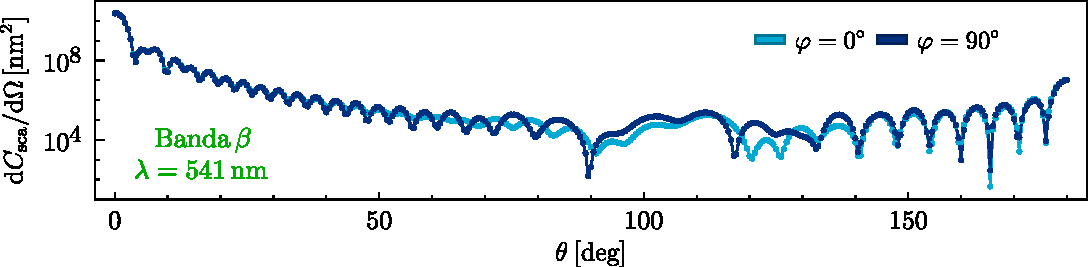
\includegraphics[width=14cm]{../../Figuras/4-Resultados/linearplot541FF_EriSano.pdf}\vspace{-0.1cm}
	\caption{Sección transversal diferencial de esparcimiento $\dd{C_{\text{sca}}}/\dd{\Omega}$ en función de $\theta$ para dos cortes: $\varphi=0^{\circ}$ (puntos azules claro) y $\varphi=90^{\circ}$ (puntos azules oscuro). La línea continua que une los puntos es una guía visual.}
	\label{fig:FF_cartesian_541_health}
\end{figure}
%
En la Fig.~\ref{subfig:FF_573_health} se muestra la sección transversal diferencial de esparcimiento $\dd{C_{\text{sca}}}/\dd{\Omega}$, así como su representación polar [Fig. \ref{subfig:FF_polar_541_health}] para los cortes $\varphi=0^{\circ}$ y $\varphi=90^{\circ}$ para $\lambda=573$~nm. En la Fig. \ref{fig:FF_cartesian_573_health} se muestra la representación cartesiana de $\dd{C_{\text{sca}}}/\dd{\Omega}$ para los cortes $\varphi=0^{\circ}$ y $\varphi=90^{\circ}$ para $\lambda=573$ nm. Al igual que para las longitudes de onda de 431 y 541 nm, el esparcimiento se concentra predominantemente en la región frontal. En este caso, el factor de anisotropía alcanza su valor máximo ($g=0.99$), lo que indica una mayor direccionalidad del esparcimiento hacia adelante. Asimismo, las principales diferencias entre los cortes $\varphi=0^{\circ}$ y $\varphi=90^{\circ}$ continúan localizándose en la región lateral, donde la correlación aumenta a $r=0.71$, valor superior al obtenido para $\lambda=541$ nm, aunque todavía inferior al observado en las regiones frontal y de retroesparcimiento. Este comportamiento es consistente con el incremento de la contribución del esparcimiento frontal al aumentar la longitud de onda, reflejado tanto en el aumento del factor de anisotropía como en las contribuciones integradas resumidas en la Tabla~\ref{table:431_val_health}.
	%
\begin{figure}[tb]
	\centering
	\sidesubfloat[First image]{\hspace{-0.5cm}{	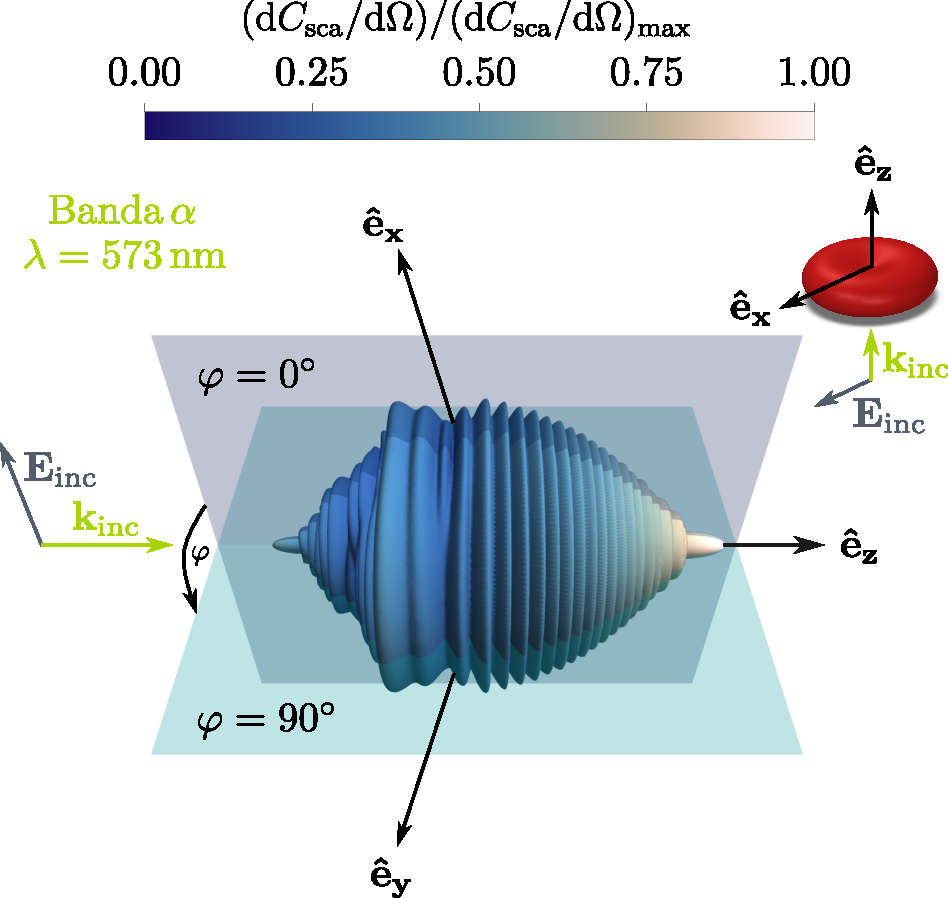
\includegraphics[width=7.3cm]{../../Figuras/4-Resultados/FFdistribution573_EriSano.pdf}\label{subfig:FF_573_health}}}\hspace{0.1cm}
	\sidesubfloat[Second image]{\hspace{-0.5cm}{
			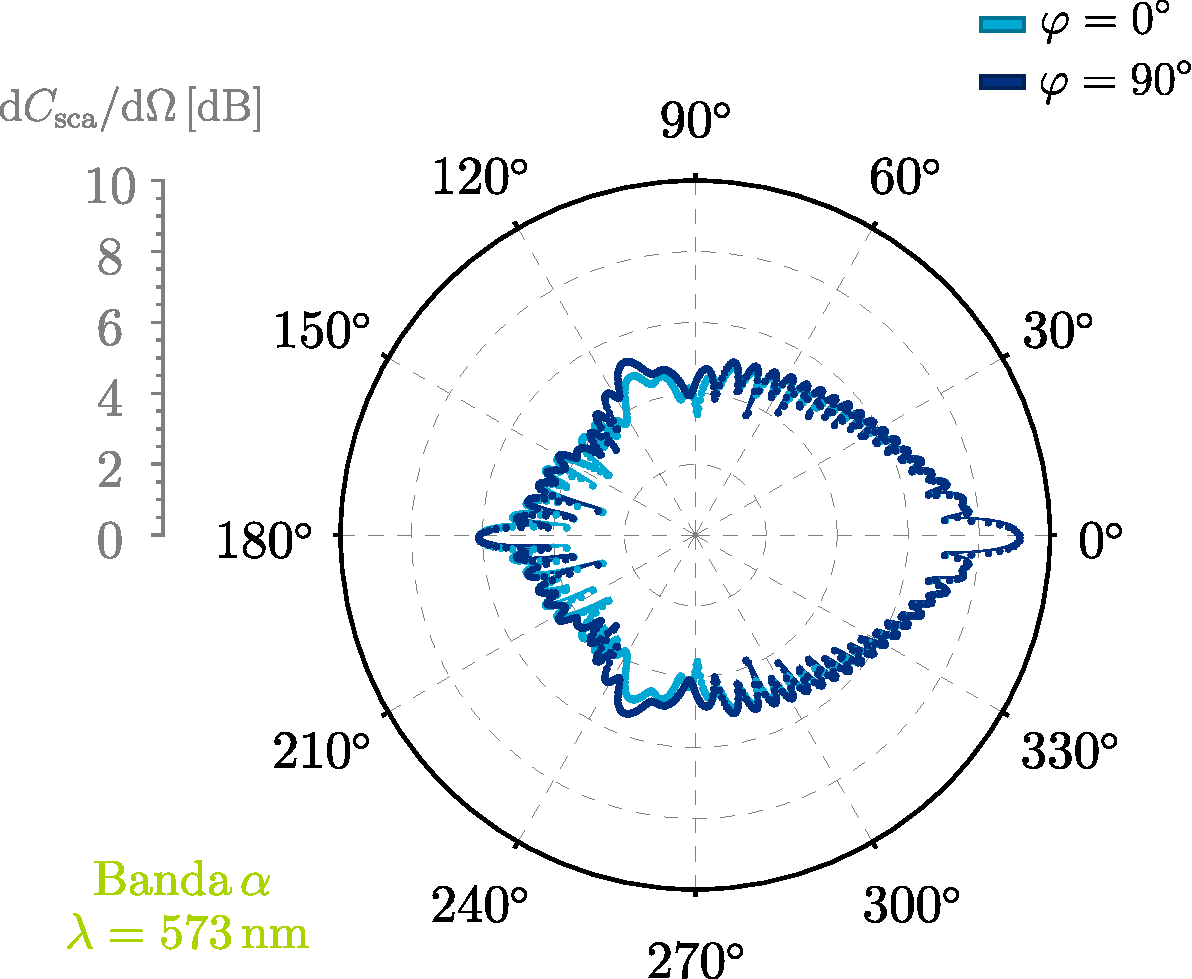
\includegraphics[width=8cm]{../../Figuras/4-Resultados/polarplot573FF_EriSano.pdf}\label{subfig:FF_polar_573_health}}}\vspace{-0.1cm}
	\
	\vspace{0.1cm}
	\caption{\textbf{a)} Sección transversal diferencial de esparcimiento $\dd{C_{\text{sca}}}/\dd{\Omega}$ normalizada respecto a su valor máximo para una longitud de onda $\lambda=573$ nm en función del ángulo de esparcimiento $\theta$ y del ángulo $\varphi$ para un eritrocito sano. Se identifican dos planos $\varphi=0^{\circ}$ en azul claro y $\varphi=90^{\circ}$ en azul oscuro. \textbf{b)} Sección transversal diferencial de esparcimiento $\dd{C_{\text{sca}}}/\dd{\Omega}$ en decibeles en función de $\theta$ para dos cortes: $\varphi=0^{\circ}$ (puntos azules claro) y $\varphi=90^{\circ}$ (puntos azules oscuro). La línea continua que une los puntos es una guía visual.}
	\label{fig:FF_573_health_1}
\end{figure}
%

	%
\begin{figure}[h!]
	\centering
	
			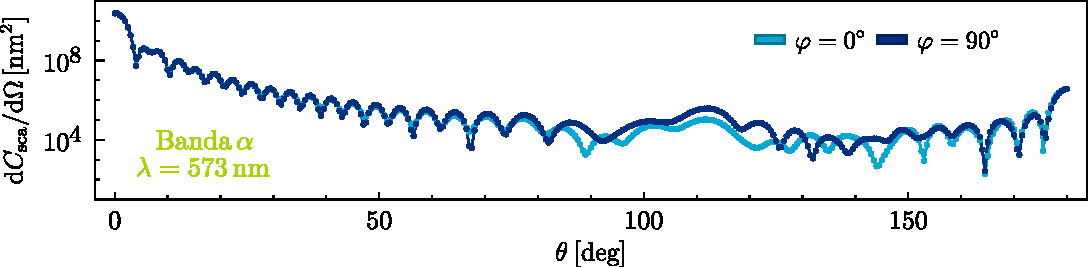
\includegraphics[width=14cm]{../../Figuras/4-Resultados/linearplot573FF_EriSano.pdf}\vspace{-0.1cm}
	\caption{Sección transversal diferencial de esparcimiento $\dd{C_{\text{sca}}}/\dd{\Omega}$ en función de $\theta$ para dos cortes: $\varphi=0^{\circ}$ (puntos azules claro) y $\varphi=90^{\circ}$ (puntos azules oscuro). La línea continua que une los puntos es una guía visual.}
	\label{fig:FF_cartesian_573_health}
\end{figure}
%